% ------------------------------------------------------------------------
%                             Capítulo 3
% ------------------------------------------------------------------------
\chapter{Desarrollo del algoritmo \acs{ALPR}}
En este capítulo se va a tratar la estructura del algoritmo \ac{ALPR}, así como su desarrollo en el entorno Matlab. 

La tarea que debe realizar este algoritmo es claramente divisible en tres tareas más simples. Primero, se debe encontrar la zona de la imagen donde se encuentra la matrícula. Una vez aislada esa parte de la imagen, se debe extraer cada uno de los dígitos que componen el número de matrícula. Por último, se deben analizar cada uno de los dígitos para determinar con qué carácter se corresponden.

\section{Detección del recuadro de la matrícula}
Para diferenciar el recuadro de la matrícula del resto de la fotografía se han utilizado dos elementos comunes a la mayoría de las matrículas: 
\footnote{Debido a la corta duración del \ac{TFG} el trabajo se centrará exclusivamente en matrículas europeas no compactas.}

\begin{itemize}
\item Un recuadro con unas dimensiones aproximadas conocidas.
\item Letras negras sobre un fondo blanco.
\end{itemize}

El diagrama de flujo del proceso realizado se puede ver en la \reff{diagrecuadro}. A continuación, vamos a analizar en detalle cada una de las fases.

\begin{figure}[!h]
\centering
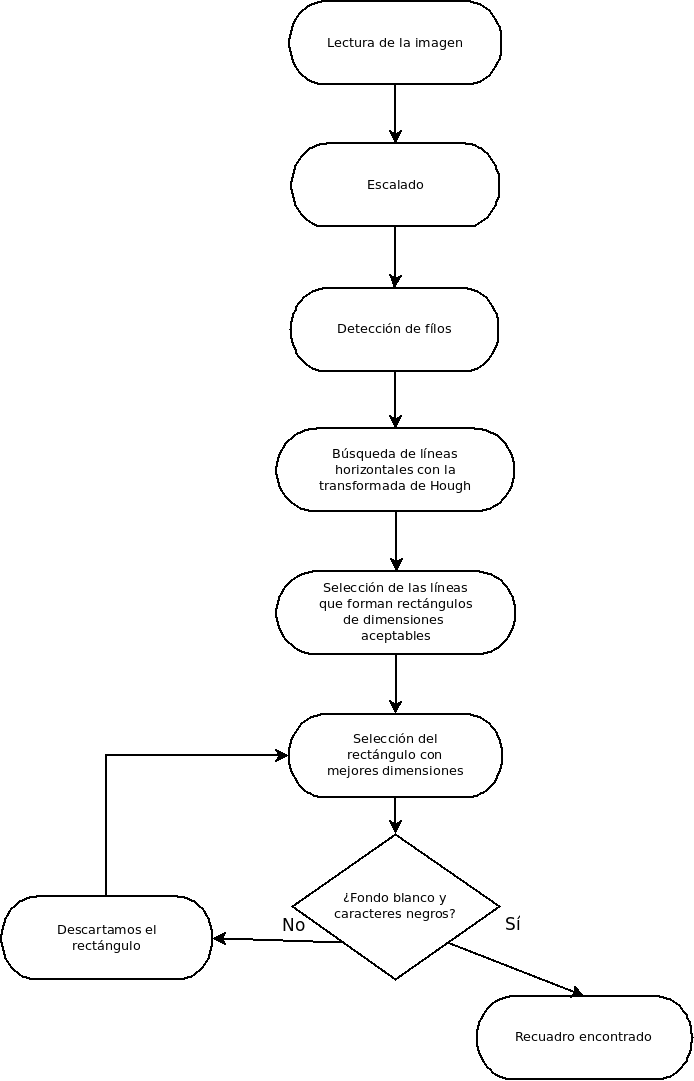
\includegraphics[width=12cm]{DiagramaProyecto.png}
\caption{\small{Diagrama de flujo para la búsqueda del recuadro.}}
\label{diagrecuadro}
\end{figure} 

\subsection{Escalado}
El primer paso consiste en aplicarle un escalado a la imagen, puesto que la cámara de 5 Mpx con la que se ha trabajado tiene demasiada resolución y capta detalles innecesarios que sólo empeoran el resultado. Para esta aplicación se empleará un factor de escalado de tres. El efecto puede verse en la \reff{figescalado}.

\begin{figure}[!h]
\centering \subfigure[Original]{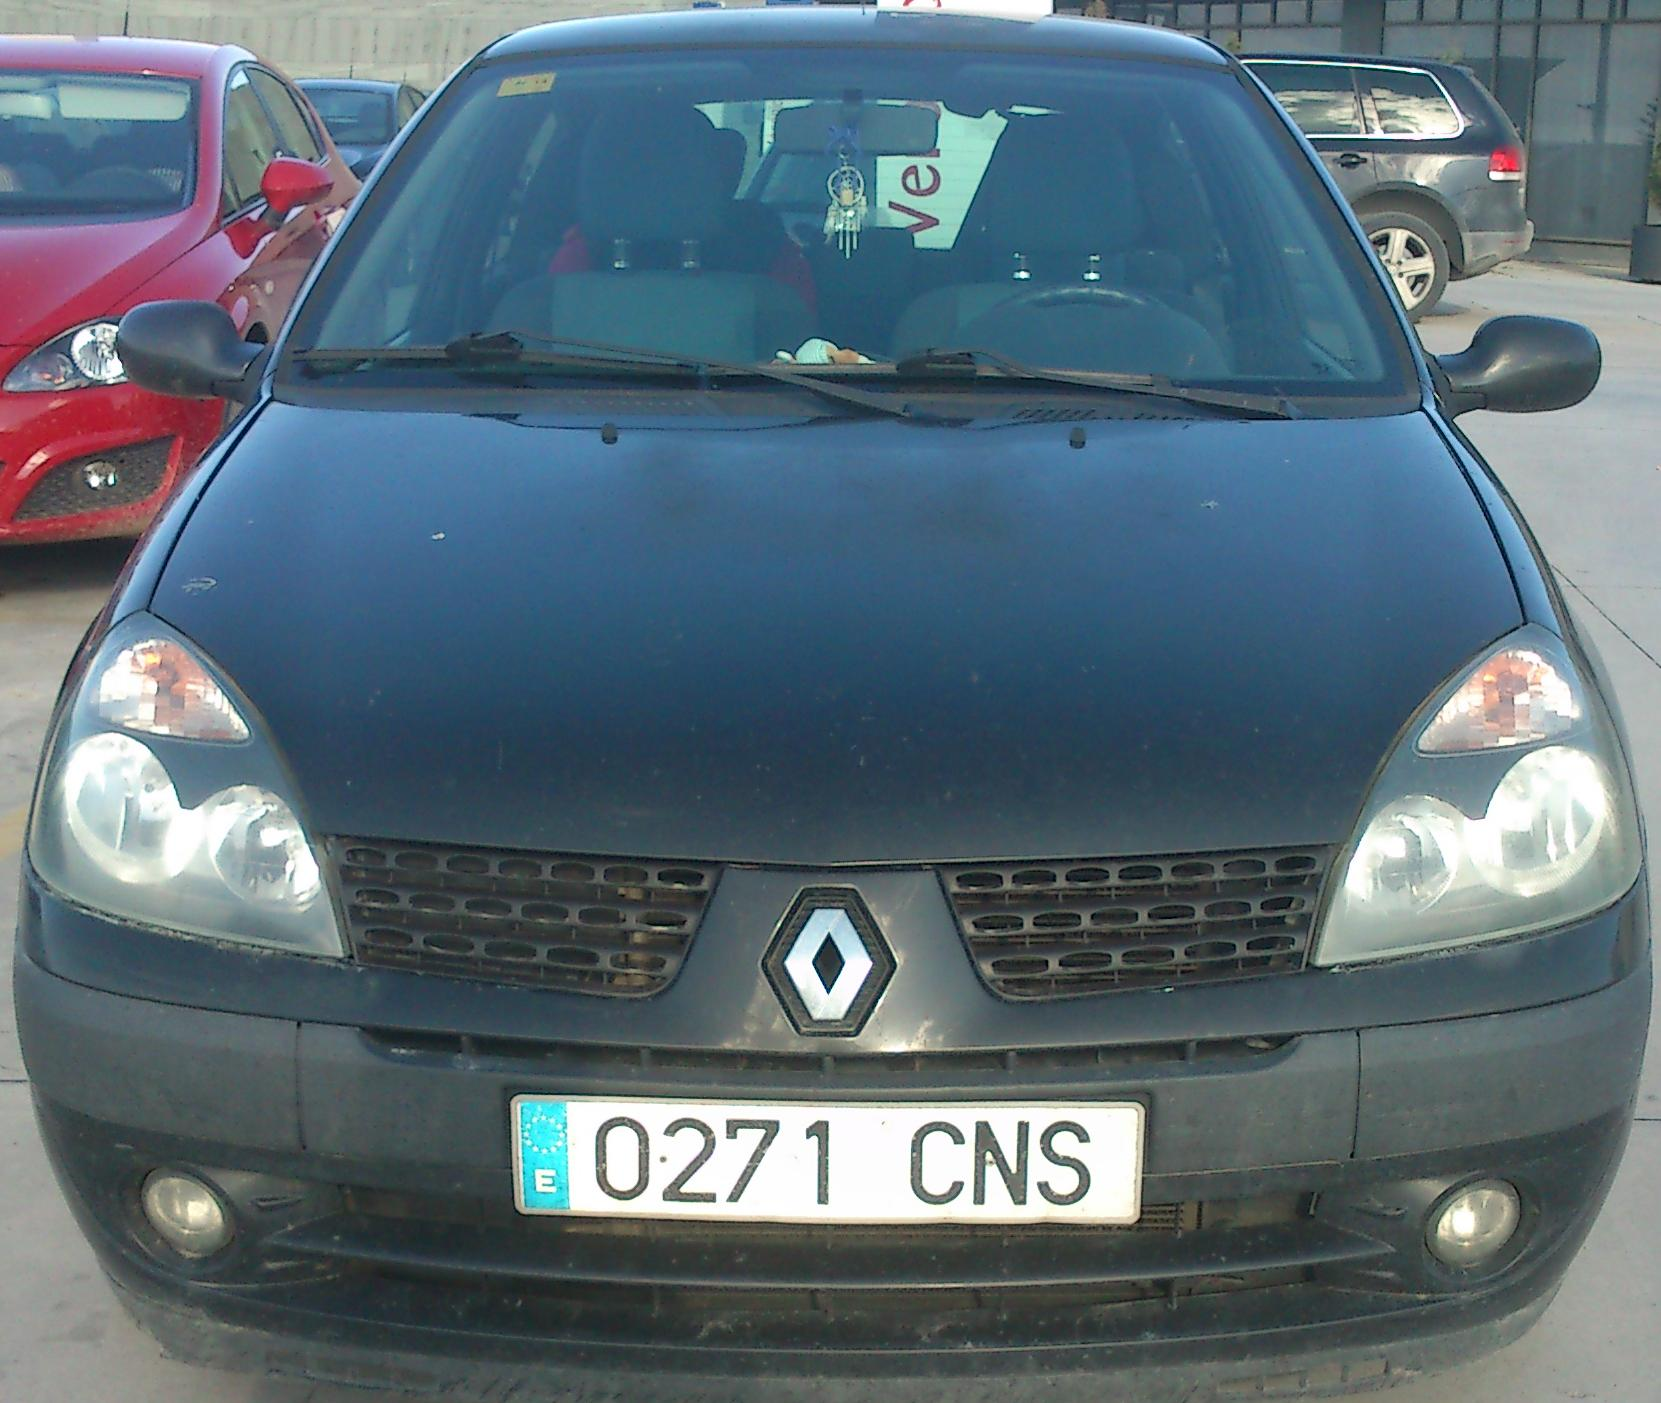
\includegraphics[width=9cm]{Original.png}}
\subfigure[Reducida]{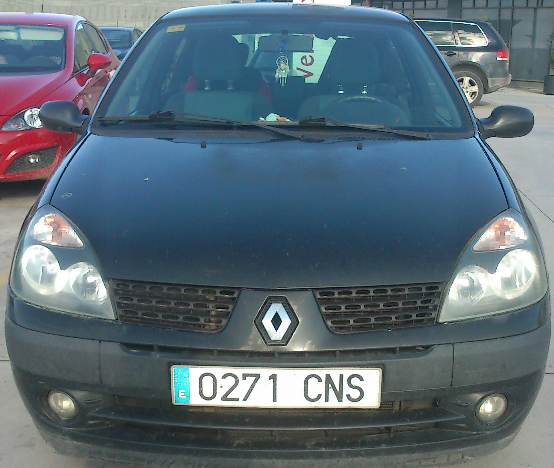
\includegraphics[width=3cm]{Reducida.png}}
\caption{\small{Efecto del escalado sobre la imagen.}} \label{figescalado}
\end{figure}

La reducción del tamaño de la imagen también trae consigo una reducción del tiempo que el algoritmo tarda en procesarla. Esto resulta particularmente importante puesto que el objetivo último de este \ac{TFG} es ejecutar el algoritmo en un sistema empotrado, donde la capacidad de proceso es muy limitada.

\subsection{Detección de contornos}\label{Canny}
La detección de contornos es un paso fundamental para la búsqueda de líneas rectas. Dicho proceso lo llevamos a cabo mediante el algoritmo de Canny. El funcionamiento del mismo y los motivos de su elección ya se trataron en el apartado \ref{canny}.\\

En Matlab se implementa mediante la función

\begin{lstlisting}
edge(Img, canny', [T1,T2], sigma);
\end{lstlisting}

\newpage 
Donde:
\begin{itemize}
\item \textbf{T1 y T2} se corresponden con los umbrales usados por el algoritmo para determinar los contornos. En esta aplicación se ha elegido [\emph{T}1 , \emph{T}2]=[0.12 ,  0.3].

\item \textbf{sigma} es la desviación típica del filtro gaussiano utilizado por el algoritmo para eliminar el ruido de la imagen. En este caso se empleará $sigma=3$.
\end{itemize}

La elección de los valores finales se ha realizado a partir de pruebas sobre distintas imágenes con diferentes condiciones de luminosidad y color; buscando reducir al máximo los detalles de la imagen sin perder las líneas que marcan la placa de matrícula. Los valores por los que finalmente se ha optado son aquellos que mejores resultados han dado en las situaciones de buena luminosidad.\footnote{Se entiende por buena luminosidad una luminosidad uniforme y sin destellos en la parte de la matrícula.}\\

El resultado del algoritmo con los parámetros finales se muestra en la \reff{Cannyfinal}


\begin{figure}[!h]
\centering
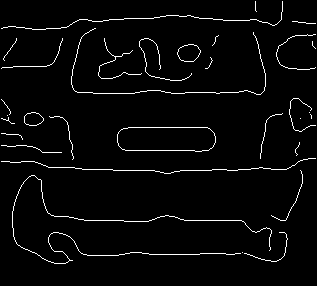
\includegraphics[width=6cm]{EjemploCanny.png}
\caption{\small{Efecto de la función Canny con los parámetros seleccionados.}}
\label{Cannyfinal}
\end{figure}

A continuación, se analizará el efecto que produce sobre los resultados la variación de estos parámetros.\\

Los umbrales \textbf {T} definen cómo de brusca ha de ser la discontinuidad en la intensidad de la imagen. Un valor demasiado pequeño resultaría en un excesivo número de contornos, lo que dificultaría la elección de los contornos que forman la matrícula; mientras que un valor demasiado grande provocaría que las líneas de la matrícula no fueran detectadas.  El efecto de los cambios sobre este parámetro puede observarse en la \reff{CannyT}.

\begin{figure}[!h]
\centering \subfigure[Umbral Bajo.]{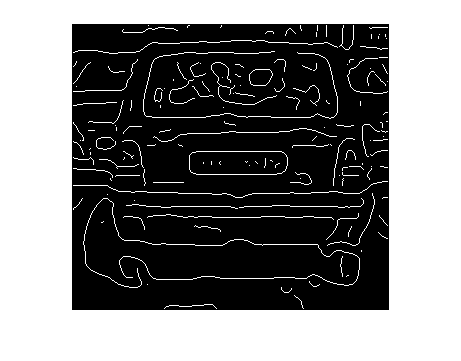
\includegraphics[width=6cm]{Tbajo.png}}
\subfigure[Umbral Alto.]{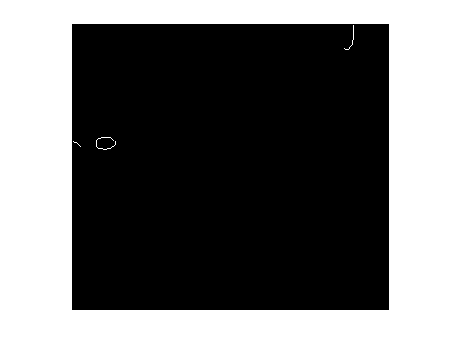
\includegraphics[width=6cm]{Talto.png}}
\caption{\small{Efecto de la modificación del parámetro T.}} \label{CannyT}
\end{figure} 

En la imagen (a) se define un umbral demasiado bajo, por lo que en la imagen aparecen muchos contornos innecesarios, que perjudican el funcionamiento del algoritmo; mientras que en la imagen (b) se utiliza un umbral demasiado alto, lo que resulta en la desaparición del contorno de la matrícula.\\


El valor de \textbf{sigma} controla el difuminado que se le aplica a la imagen antes de buscar los contornos. Un valor demasiado pequeño ocasionaría que aparecieran demasiados detalles, que complicarían la búsqueda de las líneas. Un valor muy grande provocaría que las líneas de la matrícula desaparecieran. El efecto de los cambios sobre este parámetro pueden apreciarse en la \reff{Cannysigma}.\\

\begin{figure}[!h]
\centering \subfigure[Sigma Baja.]{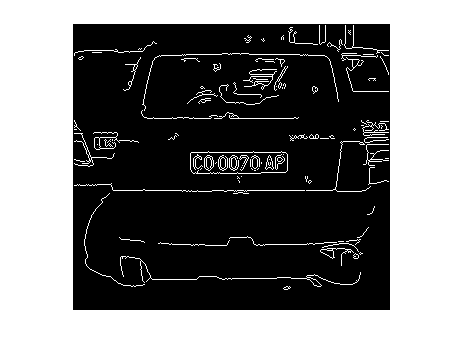
\includegraphics[width=6cm]{sigmabaja.png}}
\subfigure[Sigma Alta.]{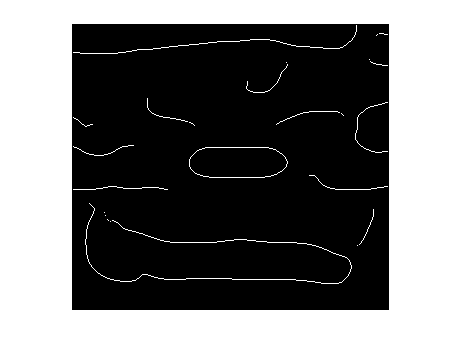
\includegraphics[width=6cm]{sigmaalta.png}}
\caption{\small{Efecto de la modificación del parámetro Sigma.}} \label{Cannysigma}
\end{figure} 

En la imagen (a) se utiliza un valor de \textbf{sigma} muy bajo, por lo que los contornos tienen demasiado detalle. En cambio, en la imagen (b) se ha usado un valor de \textbf{sigma} muy alto, por tanto, el contorno de la matrícula ha perdido su forma original.

\subsection{Búsqueda de las líneas}\label{Hough}
La forma más sencilla de separar la placa de matrícula del resto de la imagen consiste en buscar las dos líneas horizontales que la delimitan usando la transformada de Hough, cuyo funcionamiento se explico en el apartado \ref{hough}\\

En Matlab se implementa la detección de lineas mediante la transformada de Hough con las siguientes funciones:

\begin{lstlisting}
[H, theta, rho] = hough(Img, `Theta', thetaRange,`RhoResolution', rhoResolution);
P  = houghpeaks(H, NumPeaks, 'Threshold', th);
lines = houghlines(Img, theta, rho, P, 'FillGap',maxgap ,'MinLength', lmin);
\end{lstlisting}

Donde:
\begin{itemize}
\item \textbf{thetaRange} es el rango de valores del eje \emph{theta} para los que se buscarán líneas. Para esta aplicación, nos interesa ajustarlo de forma que sólo detecte líneas en dirección horizontal.

\item \textbf{rhoResolution} establece la resolución de la transformada en el eje \emph{rho}. Es decir, controla cuanta variación de \emph{rho} es aceptada en una línea. Para esta aplicación se ha usado $rho~=~7$(píxeles).

\item\textbf{NumPeaks} se corresponde con el máximo número de picos devueltos. En caso de que encuentre más picos que los configurados devolverá los más grandes. En esta aplicación se ha configurado con un número arbitrariamente grande $NumPeaks~=~99$ para tener la certeza de no perder las líneas de la matrícula.

\item\textbf{th} indica el número de líneas que deben coincidir en un punto del plano $\theta\rho$, para ser considerado línea. En esta aplicación se usará el valor por defecto que emplea Matlab $th~=~0.4*max(H)$.

\item\textbf{maxgap} establece la discontinuidad máxima que puede contener una línea para no ser considerada como dos lineas distintas. En esta aplicación se utilizará\\ $maxgap~=~anchoImg/50$.

\item\textbf{lmin} indica la longitud mínima en píxeles que debe tener una línea para ser considerada por el algoritmo. En esta aplicación se emplea $lmin~=~anchoImg/5$.

\item\textbf{H} es una matriz devuelta por la función \emph{hough} que indica el número de líneas que coinciden para cada píxel en el plano~$\theta\rho$. El tamaño de dicha matriz dependerá de la resolución de theta y rho que se haya configurado.

\item\textbf{theta y rho} son los vectores que contienen los ejes theta y rho, usados para crear la matriz \emph{H}.

\item\textbf{P} es la matriz que contiene las coordenadas de cada pico encontrado. Las coordenadas vienen dadas como fila y columna de la matriz \emph{H}.

\item\textbf{lines} es un array de estructuras que contiene la información de cada línea encontrada por la función \emph{houghlines}.
\end{itemize}

La elección de los valores finales se ha determinado, de nuevo, tras realizar pruebas en distintas imágenes; buscando los conjuntos de parámetros que obtengan resultados satisfactorios en la mayoría de ellas. Se entiende por buen resultado la aparición del menor número posible de líneas, pero siempre localizando las de la matrícula. El resultado con los parámetros finales puede observarse en la \reff{Houghfinal}.

\begin{figure}[!h]
\centering
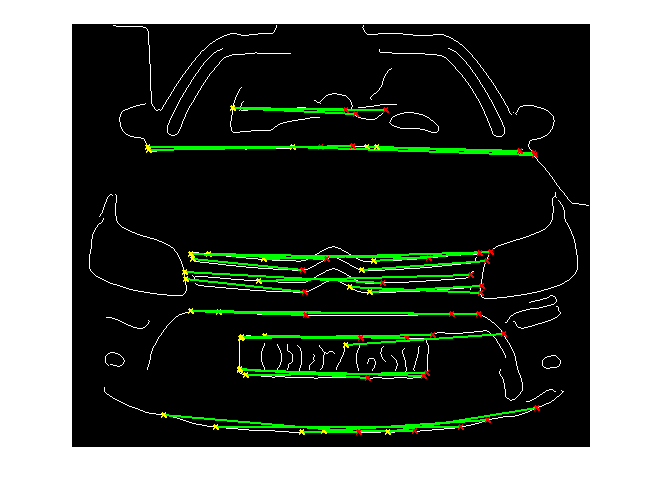
\includegraphics[width=6cm]{EjemploHough.png}
\caption{\small{Detección de líneas con los parámetros seleccionados.}}
\label{Houghfinal}
\end{figure}

A continuación, se estudia el efecto de la variación y el efecto de estos parámetros.\\

Un valor demasiado grande del parámetro rhoResolution provoca que una gran cantidad de líneas sean aceptadas como válidas; mientras que un valor demasiado bajo produciría que no se detectaran las líneas de la matrícula si éstas contienen alguna imperfección. El efecto de la variación del parámetro puede verse en la \reff{cambiorho}. 

\begin{figure}[!h]
\centering \subfigure[Rho Baja.]{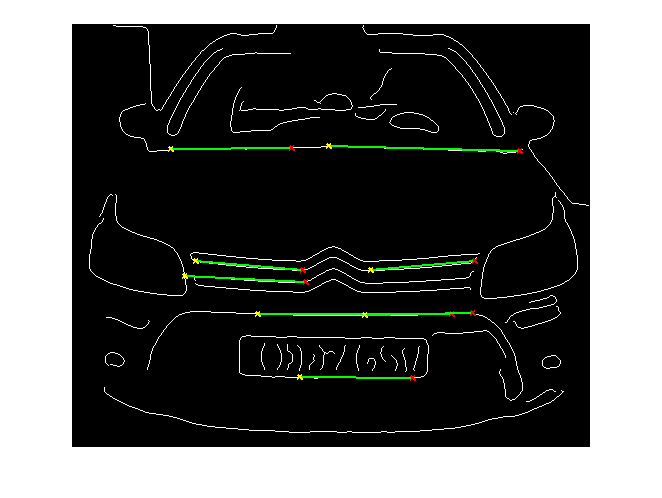
\includegraphics[width=6cm]{rhobaja.png}}
\subfigure[Rho Alta.]{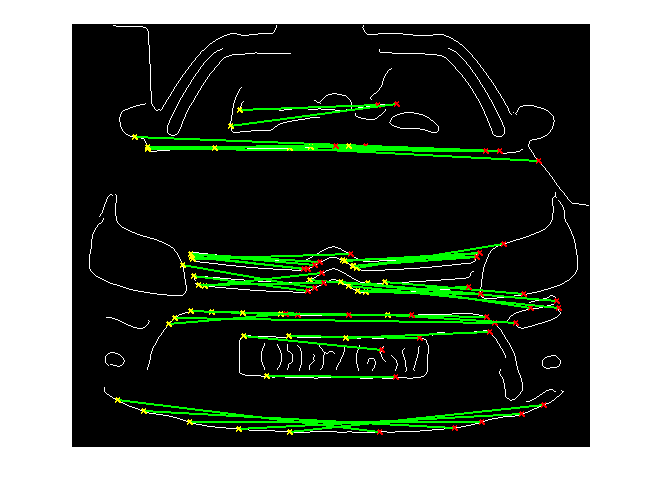
\includegraphics[width=6cm]{rhoalta.png}}
\caption{\small{Efecto de la modificación del parámetro rho.}} \label{cambiorho}
\end{figure} 

La imagen (a) utiliza un valor de rhoResolution demasiado bajo: no se detectan las líneas de la matrícula, ya que no son completamente rectas. Sin embargo, en la imagen (b) se utiliza un valor demasiado alto, lo que resulta en la aparición de un gran número de líneas en la carrocería. Además, al tener tan baja resolución en el eje, no es capaz de diferenciar los píxeles que pertenecen a los contornos de los dígitos de los pertenecientes al borde de la matrícula, lo que produce resultados inesperados. \\

El parámetro \textbf{th} indica lo marcada que debe estar una línea para ser detectada. Se ha optado por dejarlo con el valor por defecto que usa el algoritmo en Matlab.\\

El parámetro \textbf{maxgap} configura la discontinuidad que se considera aceptable en una línea. Un valor demasiado grande produciría la detección de líneas formadas, por píxeles no conectados en absoluto; mientras que un valor muy pequeño ocasionaría la fragmentación de las líneas de la matrícula si contuviesen alguna imperfección. Las consecuencias de la variación de este parámetro pueden apreciarse en la \reff{cambioMaxgap}. 

\begin{figure}[!h]
\centering \subfigure[MaxGap Bajo.]{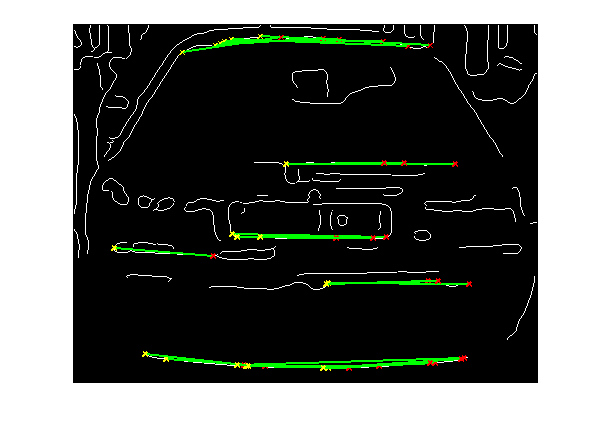
\includegraphics[width=6cm]{gapbajo.png}}
\subfigure[MaxGap Alto.]{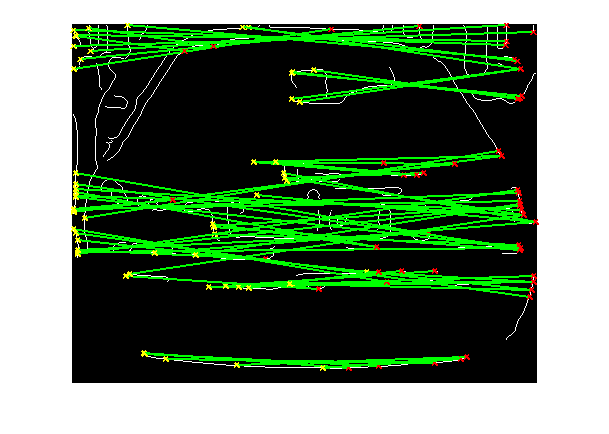
\includegraphics[width=6cm]{gapalto.png}}
\caption{\small{Efecto de la modificación del parámetro MaxGap.}} \label{cambioMaxgap}
\end{figure} 

En la imagen (a) se ha configurado el parámetro con un valor muy bajo, lo que produce que no se detecte la línea superior de la matrícula debido a una imperfección. En la figura (b) se ha configurado con un valor demasiado alto; de ahí la aparición de múltiples líneas surgidas de la conexión de contornos cercanos.  \\

El parámetro \textbf{lmin} es difícilmente configurable sin conocer la localización del sistema que implemente este algoritmo, ya que dependerá en gran medida de la distancia de los vehículos a la cámara que tome las imágenes.


\subsection{Búsqueda del recuadro de la matrícula}
Una vez obtenidas las líneas rectas, es necesario decidir qué par de líneas delimitan el rectángulo. Para ello, buscamos dos líneas que delimiten un rectángulo con las dimensiones aproximadas de una placa de matrícula. Tal y como se muestra en la \reff{dimMat}, las placas de matrícula tienen una dimensión de $520~X~110~mm$; por tanto, sólo nos interesan pares de líneas que tengan un ratio parecido.

\begin{figure}[!h]
\centering
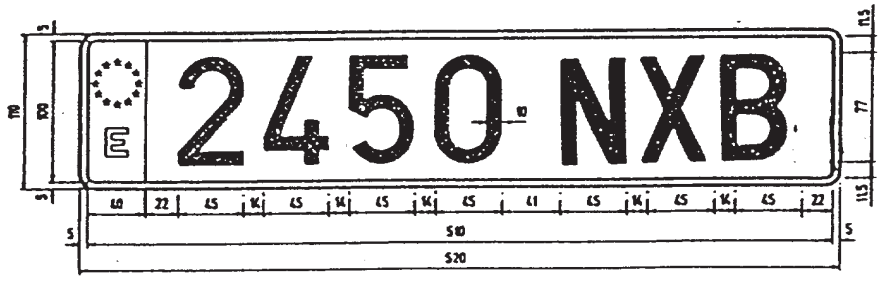
\includegraphics[width=10cm]{boe.png}
\caption{\small{Dimensiones de las placas de matrícula. Fuente:\cite{boe}}}
\label{dimMat}
\end{figure}

El proceso para buscar el rectángulo se describe a continuación:
\begin{enumerate}
\item Se analiza cada pareja de rectas, comprobando si la relación entre la longitud media en el eje x de las dos rectas y la distancia que las separa en el eje y entra en el ratio aceptable.

\item Si la pareja de rectas cumple el ratio se calcula la separación en el eje x de los dos puntos de inicio de las dos rectas, así como la separación entre los dos puntos finales.

\item Elegimos la mayor de las dos distancias calculadas en el punto anterior y la almacenamos en una matriz de distancias.
\end{enumerate}

Una vez completa la matriz distancias, el par de líneas que tenga una distancia menor será el mejor candidato para encontrar la matrícula.

\subsection{Análisis del color del candidato}
Para añadir una mayor probabilidad de acierto, comprobamos que el recuadro que seleccionamos como candidato sea en su mayoría blanco y negro, y que la relación entre píxeles negros y píxeles blancos esté dentro de unos ratios determinados. Esta comprobación ayuda a eliminar rectángulos que aparecen por la forma de la carrocería del coche o debido a alguna sombra; especialmente en coches que no sean de color blanco ni de color negro.\\

Para poder realizar esta segmentación en color se usará la representación LAB en lugar de la clásica RGB. La ventaja que ofrece la codificación LAB es que los colores pálidos están caracterizados por valores pequeños de las magnitudes A y B.

Esto quiere decir que, si se pretende separar los píxeles blancos y negros de aquellos con un color más vivo, sólo debemos aplicar un umbral a dichas magnitudes. Los píxeles que se encuentren por debajo del umbral se considerarán píxeles sin color, es decir, blancos o negros; mientras que los que se encuentren por encima se considerarán píxeles con color. 

Para distinguir píxeles blancos de píxeles negros se debe consultar el valor del parámetro L. Los colores claros se caracterizan por un valor de L bajo, mientras que los colores oscuros tienen valor de L alto.

Por tanto, es necesario establecer otro umbral para este parámetro. Para ello, se ha calculado el Threshold global de la imagen por el método Otsu. De esta forma, se calcula el nivel de gris de la imagen, y se considerarán aquellos píxeles que estén por encima del Threshold como claros y los que estén por debajo como oscuros.\\

Para más información acerca del cálculo del Threshold global con el método Otsu y de su implementación en Matlab, consultar \cite{ImgProcessMat}\\

En la \reff{ModeloLAB} podemos ver una ilustración de la representación LAB.\\

\begin{figure}[!h]
\centering
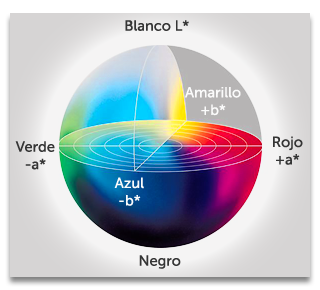
\includegraphics[width=6cm]{LAB.png}
\caption{\small{Ilustración de la representación LAB.}}
\label{ModeloLAB}
\end{figure}

Los umbrales han sido calculados tras realizar pruebas en distintas imágenes, buscando aquellos valores que ofrezcan un mejor resultado en el mayor número de imágenes posibles. Estos valores no han podido ser muy precisos, debido a que dependen en gran medida de la cantidad de píxeles de la carrocería que entren dentro del recuadro de la matrícula.\\

\begin{figure}[!h]
\centering \subfigure[Matrícula bien encuadrada.]{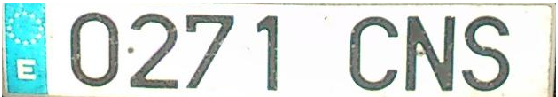
\includegraphics[width=6cm]{bienEncuadrada.png}}
\subfigure[Matrícula mal encuadrada.]{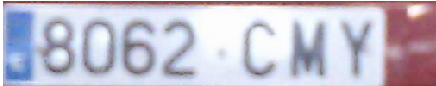
\includegraphics[width=6cm]{malEncuadrada.png}}
\caption{\small{Diferencia entre matrículas mal y bien encuadrada.}} \label{DifEncuadre}
\end{figure}

Como podemos ver en la \reff{DifEncuadre}, la imagen (a) está perfectamente encuadrada y no contiene ningún píxel correspondiente al color de la carrocería; mientras que la imagen (b) presenta un encuadre mucho peor con un gran número de píxeles de la carrocería, provocando una significativa variación en la proporción. Por tanto, para evitar que el algoritmo descarte recuadros válidos debido a un mal encuadre, los umbrales deben ser muy generosos.\\

Finalmente, los umbrales elegidos son los siguientes:
\begin{itemize}
\item Píxeles sin color: Coordenadas A y B inferiores a 150
\item Píxeles con color: Coordenadas A y B superiores a 150
\item Píxeles Blancos: Píxeles sin color con coordenada L superior al Threshold
\item Píxeles Negros: Píxeles sin color con coordenada L inferior al Threshold
\end{itemize}


Si el primer candidato cumple con los requisitos de color, será considerado como matrícula. En caso contrario, se seleccionará el segundo candidato con la mejor distancia y se volverá a probar. Este procedimiento se repetirá hasta encontrar una matrícula o hasta que se agoten los candidatos.\\

Para más información sobre el color de imágenes usando coordenadas LAB consultar \cite{matlabLAB}.

\section{Búsqueda de los dígitos}
Para encontrar los dígitos, se convierte la imagen de la matrícula a una representación binaria, donde los píxeles sólo pueden ser blancos o negros. De esta forma, se pueden extraer las distintas figuras de la imagen simplemente buscando conjuntos de píxeles negros aislados. En esta parte del algoritmo, a diferencia de la anterior, se utilizará la imagen original antes del escalado, puesto que resulta más fácil identificar los dígitos si éstos tienen una buena resolución.\\

El diagrama del algoritmo se muestra en la \reff{Diagrama2}.

\begin{figure}[!h]
\centering
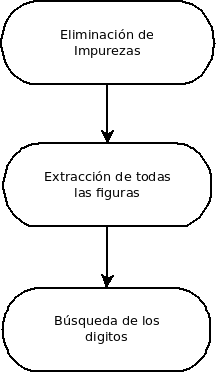
\includegraphics[width=5cm]{Diagrama2.png}
\caption{\small{Diagrama del algoritmo para buscar los dígitos.}}
\label{Diagrama2}
\end{figure}

\subsection{Eliminación de impurezas}
Tras pasar la imagen a representación binaria nos encontramos con pequeñas impurezas que ensucian la imagen y dificultan la detección de los dígitos.\\


Para eliminarlas hay que establecer un área mínima y borrar todos los conjuntos de píxeles que tengan un área menor a la establecida. Esto se puede llevar a cabo mediante la siguiente función de Matlab:

\begin{lstlisting}
matriculaSinImpurezas = not bwareaopen( not matriculaConImpurezas, areaMin)
\end{lstlisting}


Donde \textbf{areaMin} es el área mínima que deben tener los conjuntos de píxeles para no ser eliminados. Se ha establecido \textbf{areaMin} como un 5\% del área total de la matrícula.\\

Como se puede ver en la función tanto la imagen origen como el resultado de la función están negados. Esto se debe a que la función entiende por píxel activo un píxel blanco, mientras que en nuestra aplicación consideramos como píxeles activos a los píxeles negros.\\

Los resultados pueden apreciarse en la \reff{Impurezas}

\begin{figure}[!h]
\centering \subfigure[Matrícula con impurezas.]{
\includegraphics[width=6cm]{MatriculaImpurezas.png}}
\subfigure[Matrícula sin impurezas.]{
\includegraphics[width=6cm]{MatriculaSinImpurezas.png}}
\caption{\small{Resultado de la eliminación de impurezas.}} \label{Impurezas}
\end{figure}

\subsection{Extracción de todas las figuras}
El siguiente paso es identificar y extraer todas las figuras de la imagen, entre las que se encuentran los dígitos que forman el número de matrícula.

\newpage 
Extraemos las figuras con el siguiente código de Matlab:

\begin{lstlisting}
[Figuras Ne]=bwlabel( not matricula);
for n=1:Ne
	[h,w] = find(Figuras==n);
	fig(i)=matricula(min(h):max(h),min(w):max(w));
end
\end{lstlisting}

Donde:\begin{itemize}
\item \textbf{Figuras} es una matriz donde las posiciones correspondientes a los píxeles de cada una de las figuras tienen como valor un número entero distinto; mientras que los que pertenecen al fondo están marcados como 0.

\item \textbf{Ne} es el número de figuras encontradas.

\item\textbf{h} y \textbf{w} son dos variables auxiliares donde se almacenan las dimensiones de la figura encontrada.

\item\textbf{fig} es un vector donde guardan todos los resultados.
\end{itemize}

Entre las figuras encontradas, los dígitos de la matrícula no son los únicos resultados que aparecen. También se encuentras otras figuras pertenecientes a la carrocería del coche, o el símbolo de la Unión Europea, que deben ser filtrados.\\

En la \reff{Figuras} se pueden observar dos de los objetos extraídos de la matrícula representada en la \reff{Impurezas}. La imagen (a) representa un trozo del símbolo de la Unión Europea. La imagen (b) muestra uno de los números de la matrícula. Para esta aplicación, el símbolo de la Unión Europea carece de interés; por tanto, debemos ignorarlo mientras que el dígito sí debe ser procesado.

\begin{figure}[!h]
\centering \subfigure[Figura no deseada.]{
\includegraphics[width=5cm]{figuraBasura.png}}
\subfigure[Dígito de la matrícula.]{
\includegraphics[width=5cm]{figuraBuena.png}}
\caption{\small{Algunas de las figuras extraídas de la matrícula.}} \label{Figuras}
\end{figure}

\subsection{Búsqueda de los dígitos}
Por último, el algoritmo debe decidir qué resultados se corresponden con un dígito y qué resultados no. Para ello, se analizan las características de todas las figuras encontradas y se comparan con las que habitualmente se encuentran en la tipografía utilizada.\\

Las características analizadas son el área de la figura, la relación entre el alto y el ancho de la figura, la relación entre el número de píxeles blancos y negros y el número de píxeles negros.\\

Los valores de los umbrales se han decidido calculando las máximas variaciones de las características analizadas en la tipografía presente en las matrículas.\\

Pero el desgaste de las matrículas y los errores en las imágenes, tales como la inclinación o una mala iluminación, añaden imperfecciones a los dígitos extraídos. Por este motivo, ha sido necesario sumar un margen de error a los umbrales calculados. Este margen de error se ha calculado tras realizar pruebas en distintas imágenes.\\

Los umbrales resultantes son los siguientes:

\begin{itemize}
\item Área de la figura inferior al 30\% del área de la matrícula. 
\item Relación entre el alto y el ancho de la figura entre 8 y 1,3.
\item Relación entre el número de píxeles blancos y negros inferior a 4.
\item Número de píxeles negros superior a 0,4 multiplicado por la media de píxeles negros en las figuras encontradas, e inferior a 1,8 multiplicado por la media.
\end{itemize}

Las figuras que cumplan los requisitos serán consideradas como dígitos de la matrícula.\\

Un problema encontrado es que, a pesar de intentar ajustar los umbrales lo máximo posible, la figura de la Unión Europea habitualmente es reconocido como carácter válido y posteriormente identificado como una la letra `I'. Para solucionar este problema sería necesario un análisis del color de las figuras encontradas y eliminar aquellas que no sean negras.

\section{Decisión del número de matrícula}
La última tarea que debe realizar el algoritmo \ac{ALPR} es decidir con qué carácter se corresponde cada uno de los dígitos encontrados en la etapa anterior.\\

Para ello, el programa almacenará una base de datos con las imágenes de cada uno de los dígitos que componen la tipografía empleada en las matrículas. De esta forma, sólo hay que comparar cada uno de los dígitos encontrados en la imagen con cada dígito de la tipografía, y elegir aquel que nos dé una coincidencia más alta.\\

Para realizar la comparación se escalan las imágenes de forman que tengan el mismo tamaño y comprobamos píxel a píxel.\\

\begin{figure}[!h]
\centering \subfigure[Dígito encontrado.]{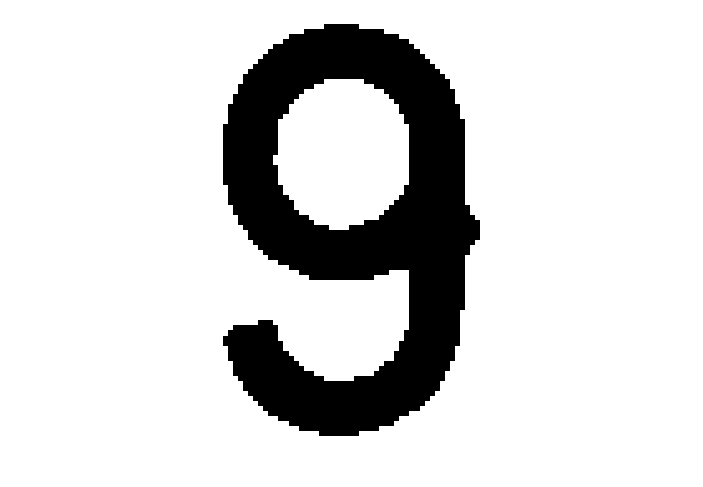
\includegraphics[width=5cm]{9.png}}
\subfigure[Dígito de la tipografía.]{
\includegraphics[width=5cm]{A.png}}
\subfigure[Resultado de la comparación.]{
\includegraphics[width=5cm]{ComparacionA_9.png}}
\caption{\small{Ejemplo de comparación erronea.}} \label{ComError}
\end{figure}

En la \reff{ComError} se puede observar el resultado de una comparación errónea. La figura (a) se corresponde con un dígito encontrado en la imagen, mientras que la figura (b) es un carácter de la tipografía. El resultado de la comparación se muestra en la figura (c). \\

Los píxeles blancos se corresponden con los píxeles que coinciden en las dos imágenes, y los negros con los que no. Puesto que no se trata del mismo dígito, el resultado de la comparación es malo.\\

En la \reff{ComCorrecta} se puede ver un ejemplo de una comparación correcta: en esta ocasión el dígito encontrado en la figura y el de la tipografía son el mismo, por tanto, la mayoría de los píxeles coinciden.

\begin{figure}[!h]
\centering \subfigure[Dígito encontrado.]{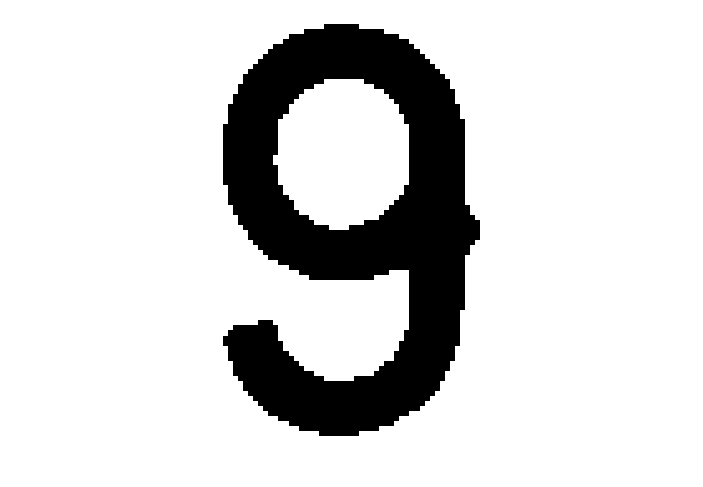
\includegraphics[width=5cm]{9.png}}
\subfigure[Dígito de la tipografía.]{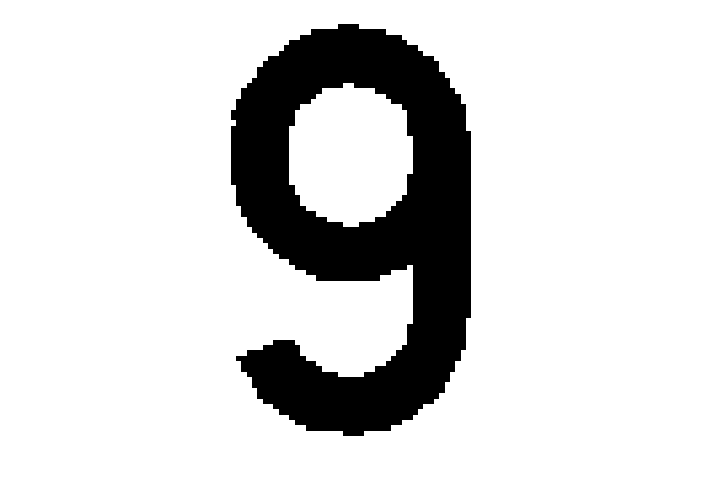
\includegraphics[width=5cm]{9_tipografia.png}}
\subfigure[Resultado de la comparación.]{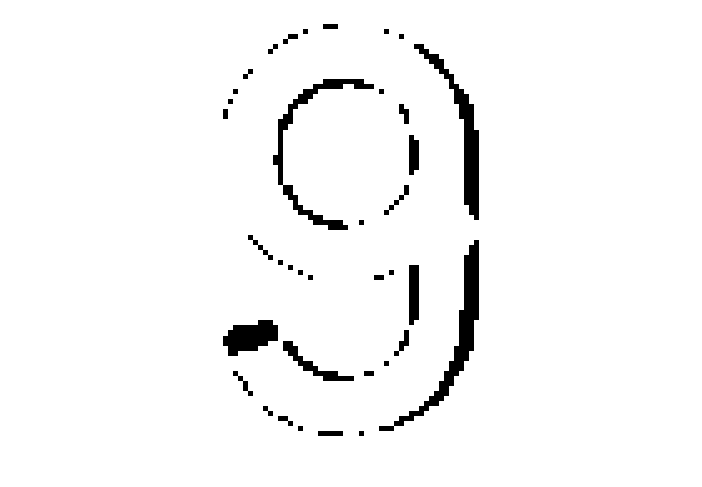
\includegraphics[width=5cm]{Comparacion9_9.png}}
\caption{\small{Ejemplo de comparación correcta.}} \label{ComCorrecta}
\end{figure}


